% \documentclass[dvipdfmx, 11pt]{beamer}
\documentclass[aspectratio=169, dvipdfmx, 11pt]{beamer} % aspectratio=43, 149, 169
\usepackage{here, amsmath, latexsym, amssymb, bm, ascmac, mathtools, multicol, tcolorbox, subfig, bookmark}

% デザイン
\usetheme{Luebeck}
\usecolortheme{orchid}
\usefonttheme{professionalfonts}
\useinnertheme{circles}
\useoutertheme{infolines}
\setbeamercolor{title}{fg=structure, bg=}
\setbeamercolor{frametitle}{fg=structure, bg=}
\setbeamertemplate{itemize item}{\small\raise0.5pt\hbox{$\bullet$}}
\setbeamertemplate{itemize subitem}{\tiny\raise1.5pt\hbox{$\blacktriangleright$}}
\setbeamertemplate{itemize subsubitem}{\tiny\raise1.5pt\hbox{$\bigstar$}}

%しおりの文字化け解消
\usepackage{atbegshi}
\ifnum 42146=\euc"A4A2
\AtBeginShipoutFirst{\special{pdf:tounicode EUC-UCS2}}
\else
\AtBeginShipoutFirst{\special{pdf:tounicode 90ms-RKSJ-UCS2}}
\fi

\setbeamertemplate{navigation symbols}{}
\renewcommand{\kanjifamilydefault}{\gtdefault}
\newcommand{\red}[1]{\textcolor{red}{#1}}
\newcommand{\green}[1]{\textcolor{green!40!black}{#1}}
\newcommand{\blue}[1]{\textcolor{blue!80!black}{#1}}

\title[Day04]{機械学習の基礎}
\subtitle{Day04}
\author[Yudai Fujimoto]{Yudai Fujimoto}
\institute[SUS]{Suwa University of Science}
\date{\today}

\begin{document}
\maketitle

\begin{frame}{目次}
    \tableofcontents
\end{frame}

\section{欠損値の処理}
\begin{frame}{欠損値の処理}
    実際のデータには様々な理由でデータの値が欠損している場合がある。
    例えば、適切な測定が行えない場合やアンケートの調査での空欄等が挙げられる。
    一般的にそうした欠損値(missing value)は空欄やNaNなどの仮の文字列で表される。
    欠損値は演算が行えないので適切な処理が必要である。
\end{frame}

\section{カテゴリデータの整形}
\begin{frame}{カテゴリデータの整形}
    これまでは数値のみのデータを扱ってきたが現実のデータにはよくカテゴリ値の特徴量が含まれる。
    カテゴリデータに関しては順序(ordinal)特徴量と名義(nominal)特徴量を区別する必要がある。
    \vspace{1em}
    \begin{itemize}
        \item 順序特徴量: 順序付けが可能
        \begin{itemize}
            \item e.g. 服のサイズ XL \(>\) L \(>\) M \(>\) S
        \end{itemize}
        \item 名義特徴量: 順序付けができない
        \begin{itemize}
            \item e.g. 服の色 赤 ? 青 ? 黄
        \end{itemize}
    \end{itemize}
    \vspace{1em}
    これらのカテゴリデータを演算可能な値に変換する必要がある。
\end{frame}

\section{正則化}
\begin{frame}{正則化}
    単純に損失関数を最小するだけではモデル複雑化し、過学習に陥りやすい。
    そこで、損失関数のモデルの複雑さを表す正則化項を追加することで、
    モデルが複雑になるのを防ぐことができる。
    具体的には大きな重みにペナルティを課し、小さな重みになることを促す。
    \vspace{2em}
    \begin{figure}[b]
        \begin{center}
        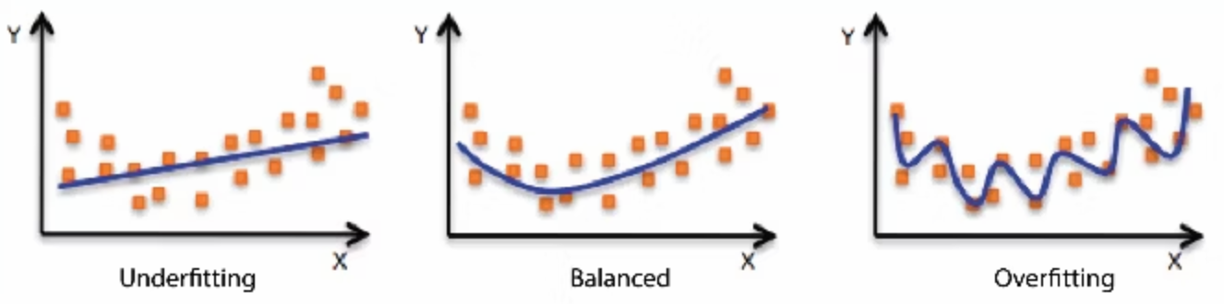
\includegraphics[width=140mm]{img/day04/fig01.png}
        \end{center}
    \end{figure}
\end{frame}

\begin{frame}{正則化}
    正則化にはL2正則化(Ridge回帰)とL1正則化(Lasso回帰)が存在する。\\
    \vspace{1em}
    L2正則化は、寄与が小さい重みを抑えることができ、正則化項は次のように定義される。
    \begin{equation*}
        L2:\lambda {\left\lVert w \right\rVert}_{2}^{2} = \lambda \sum_{j=1}^{m}w_{j}^{2}
    \end{equation*}
    \vspace{1em}
    L1正則化は、寄与が小さい重みを0にすることができ、正則化項は次のように定義される。
    \begin{equation*}
        L1:\lambda {\left\lVert w \right\rVert}_1 = \lambda \sum_{j=1}^{m} |w_j|
    \end{equation*}
    ここで、\(\lambda\)は正則化パラメータである。\(\lambda\)を調整することで、正則化の強さを調整できる。
\end{frame}

\begin{frame}{L2正則化}
    灰色の円で示している部分は正則化による重み係数の制約範囲を示している。
    しかし、損失関数は最小化したいので制約下では損失関数とL2の円の等高線が交わる箇所が最善である。\\
    このようにして、寄与が小さい重みを抑えることができる。
    \begin{figure}[b]
        \begin{center}
        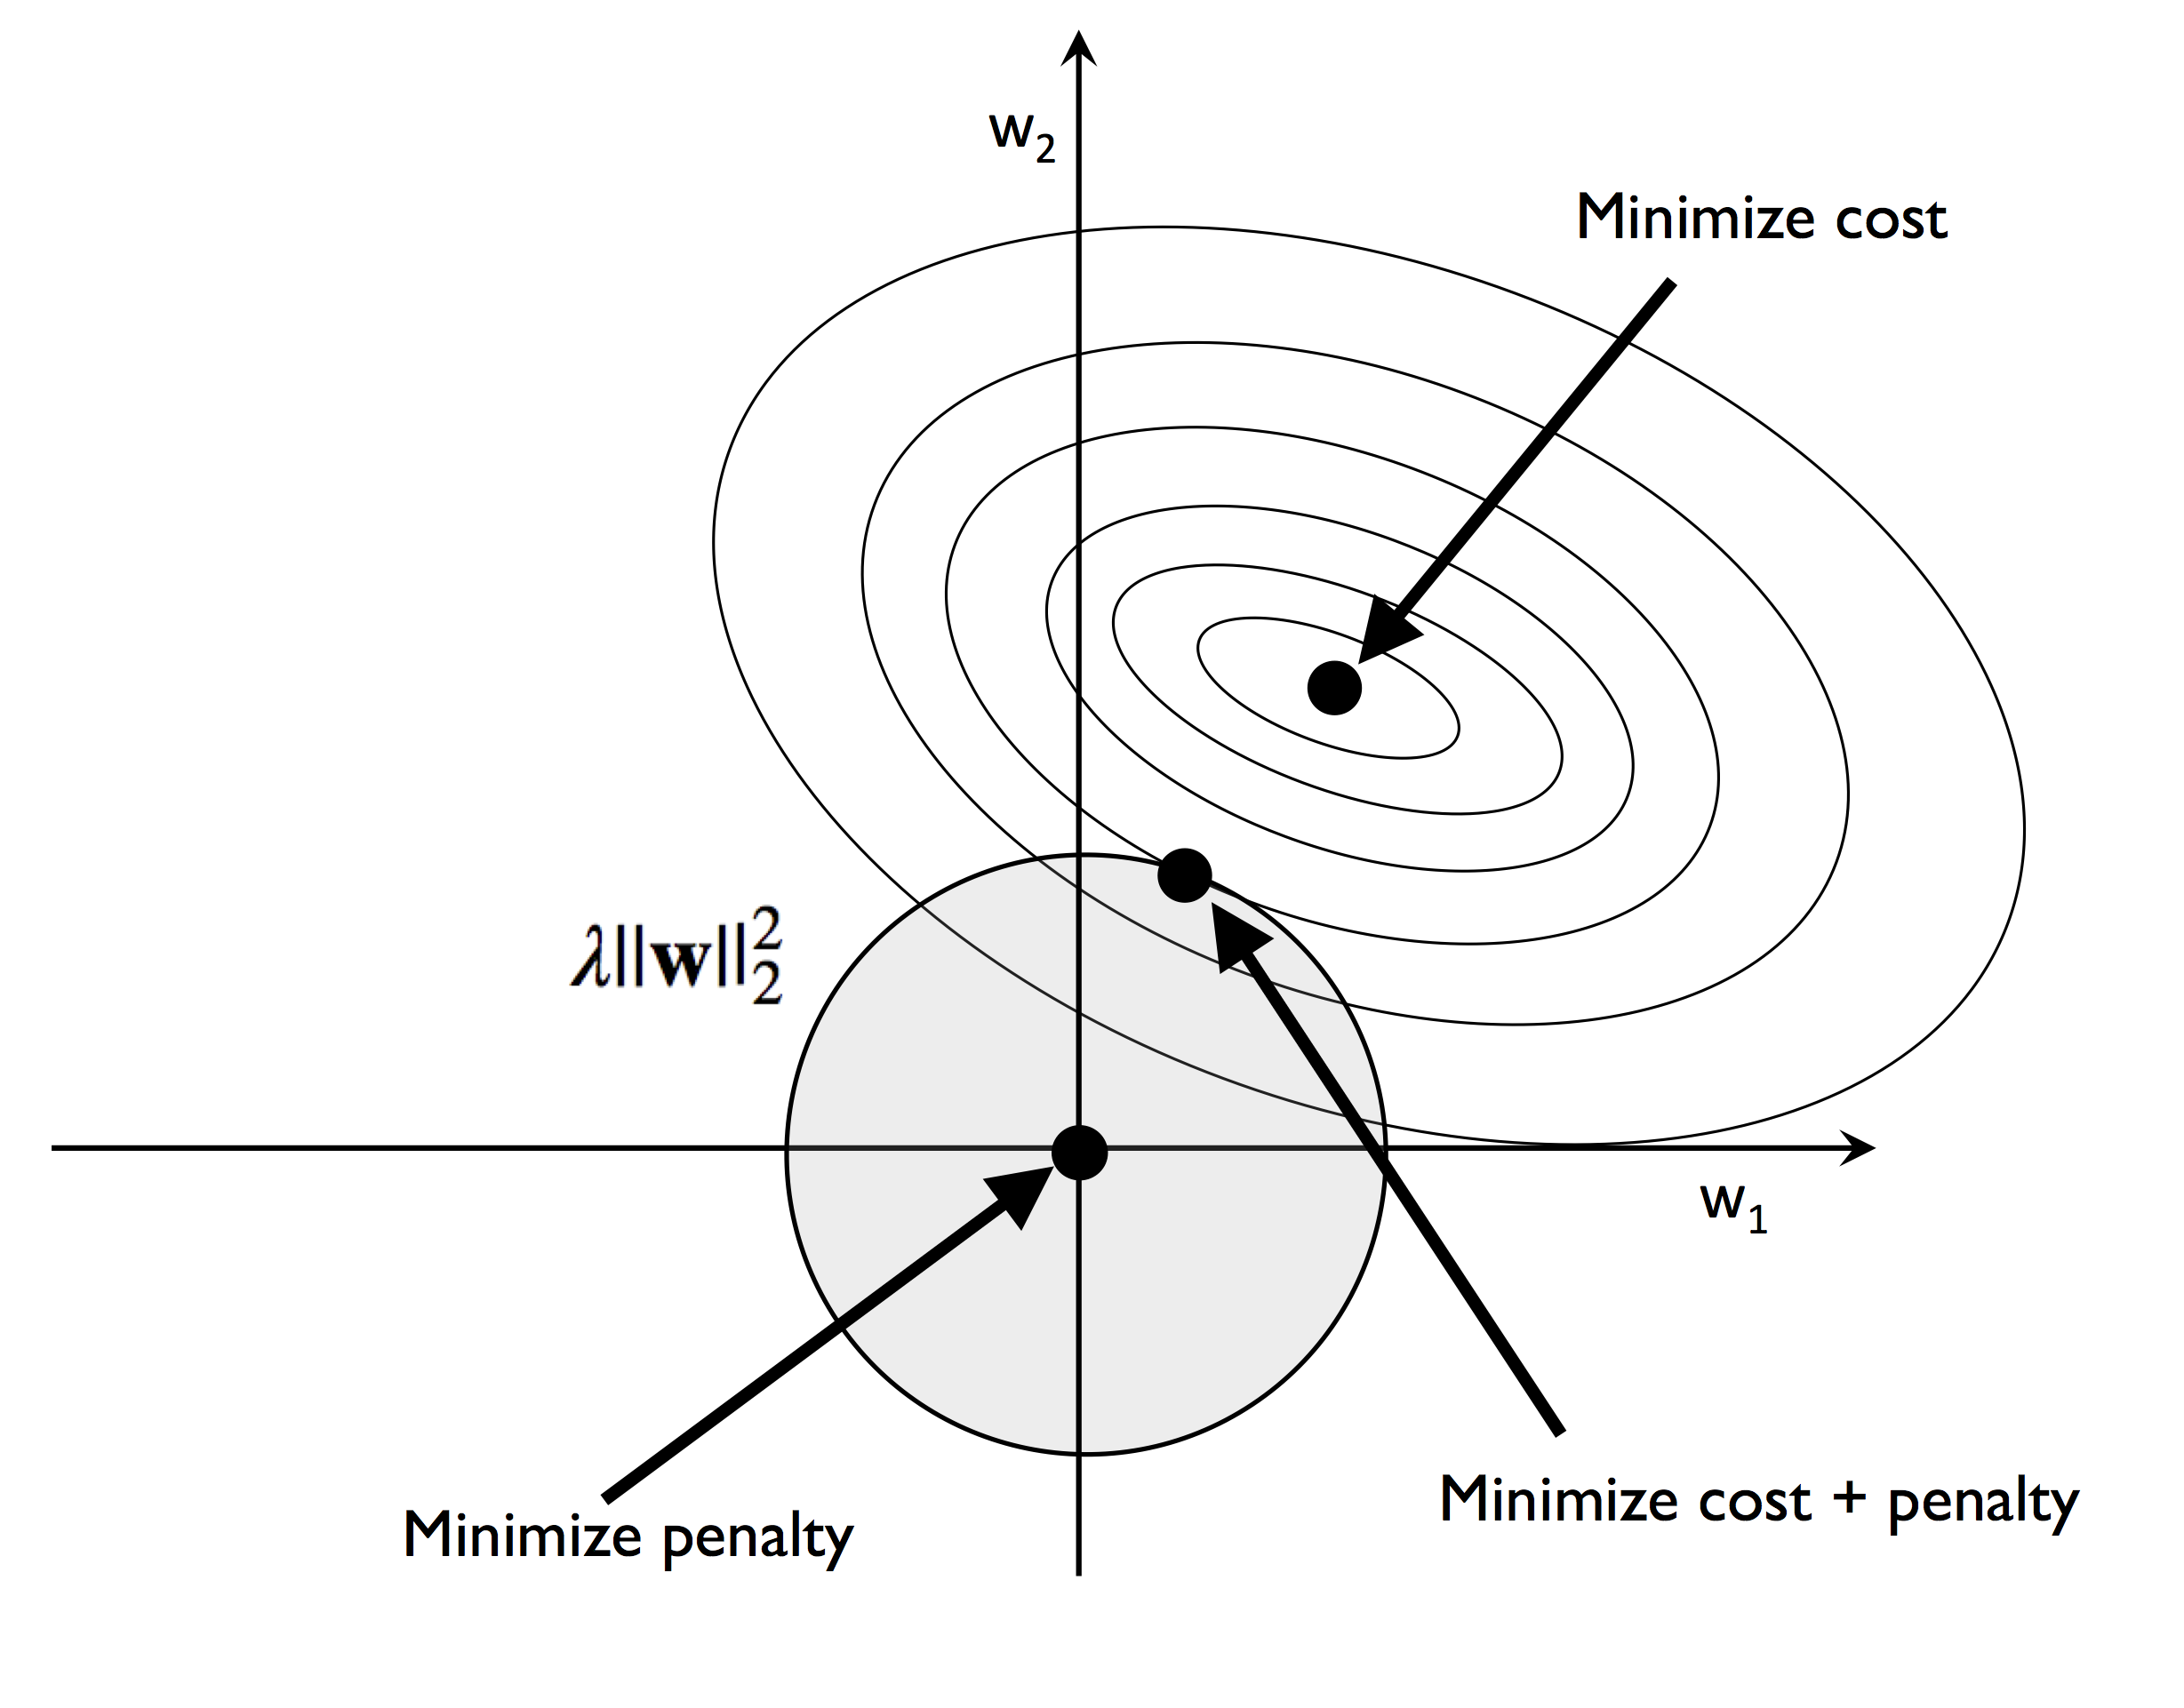
\includegraphics[width=70mm]{img/day04/fig02.png}
        \end{center}
    \end{figure}
\end{frame}

\begin{frame}{L1正則化}
    L1のペナルティは重みの絶対和であるため、制約範囲は図のようにひし形になる。\\
    ここで、損失関数の等高線はひし形の角の部分と接しやすいので、もう片方の重みを0にできる。
    このようにして、寄与の少ない重みを0にすることができる。
    \begin{figure}[b]
        \begin{center}
        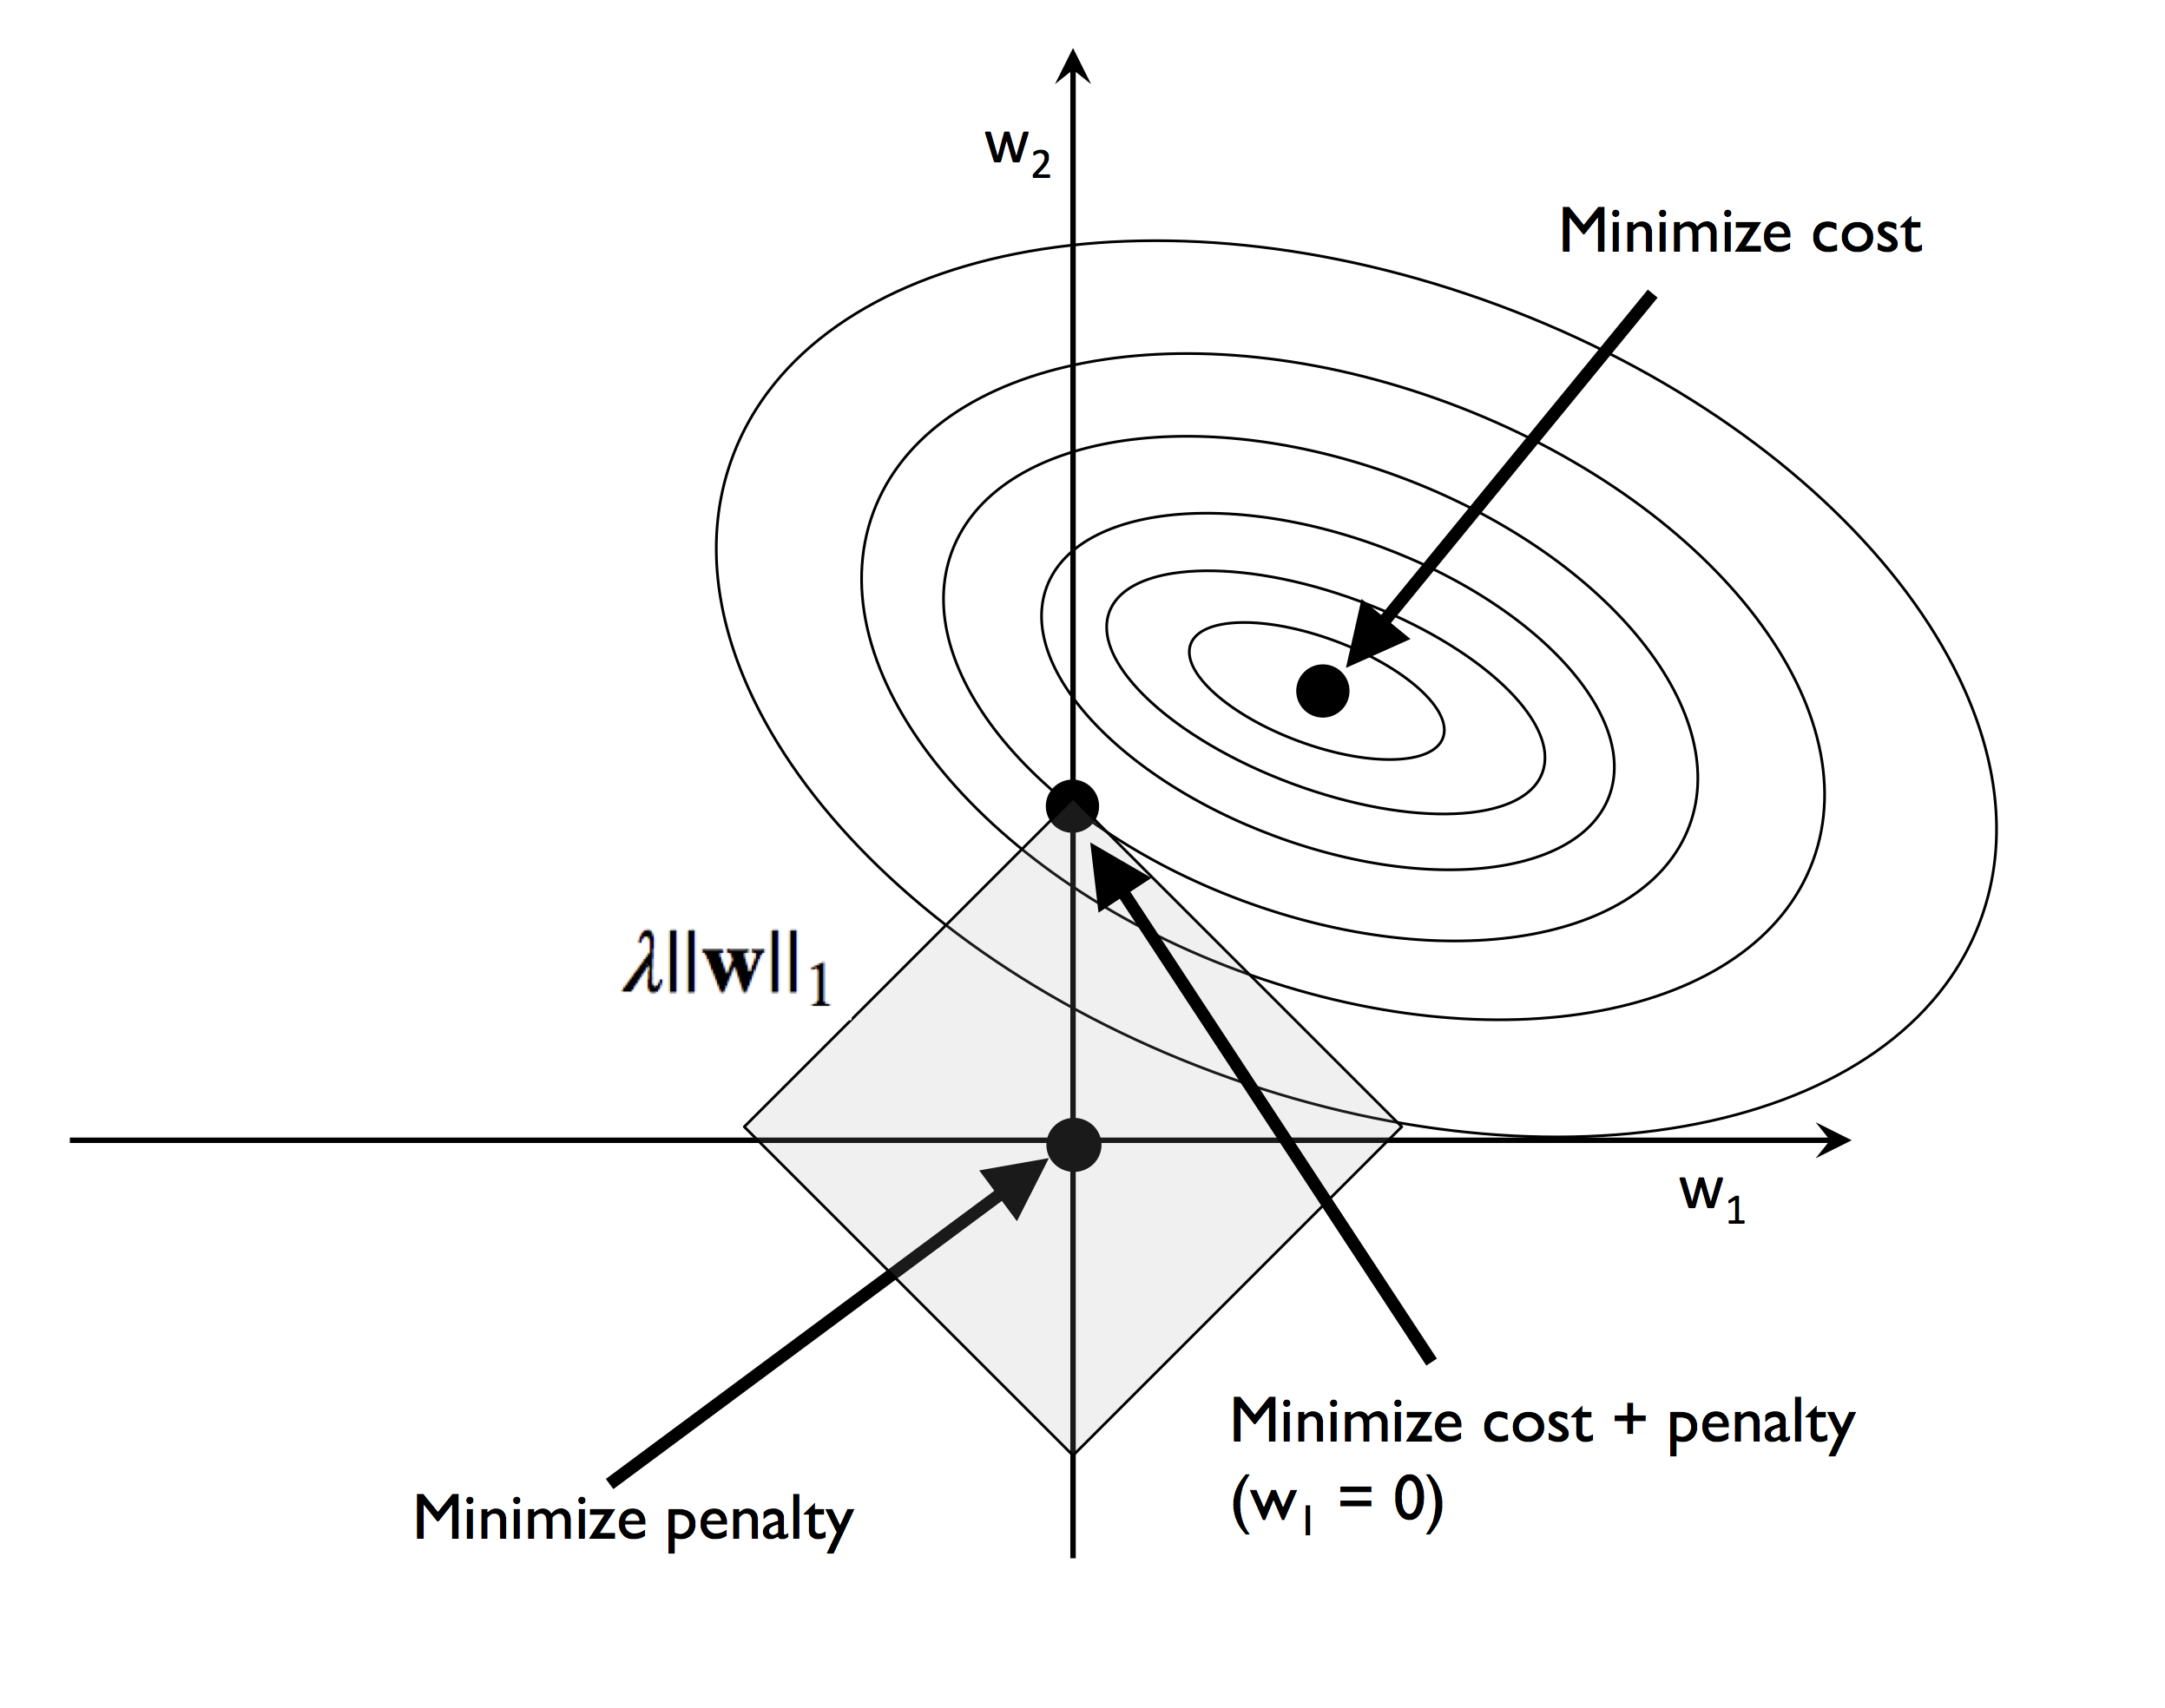
\includegraphics[width=70mm]{img/day04/fig03.png}
        \end{center}
    \end{figure}
\end{frame}

\end{document}